\section{The elephant in the Wasserstein space}\label{sec:elephant-wasserstein-space}

Our approach combines hemisphere masses with Mellin moments. By
construction, we show that the CWOLA classifier suppresses generalized
hadronization corrections up to power corrections. This assumption is
well motivated before hadronization.

\begin{figure}[t]
\centering
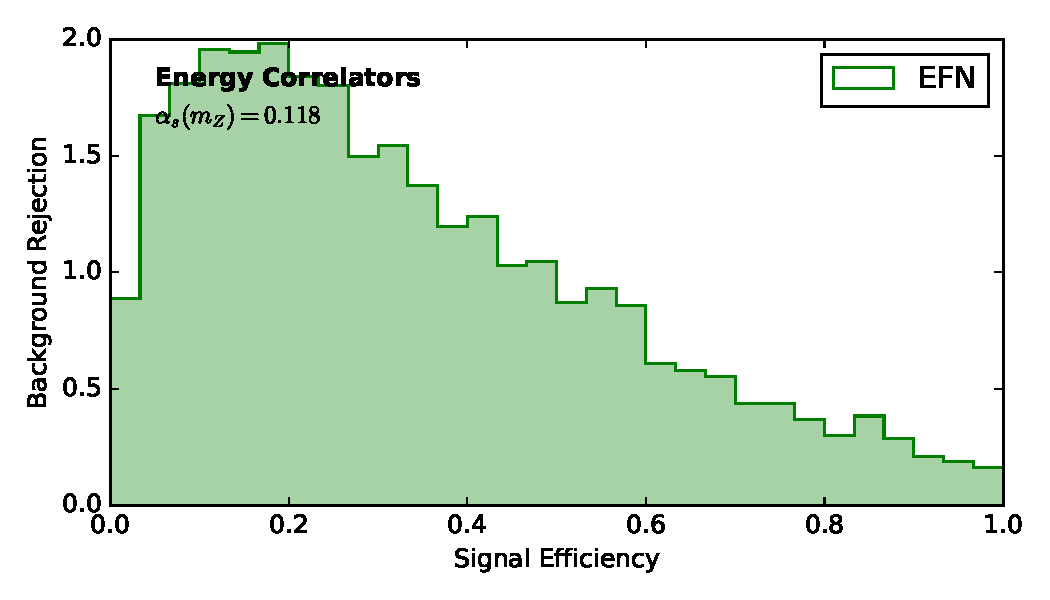
\includegraphics[width=0.9\textwidth]{figures/sudakov-ratio.pdf}
\caption{Distribution of bootstrap methods trained on simulated FCC data for Higgs plus jet production at $\sqrt{s} = 240$ GeV.}
\label{fig:sudakov-ratio}
\end{figure}

\begin{figure}[t]
\centering
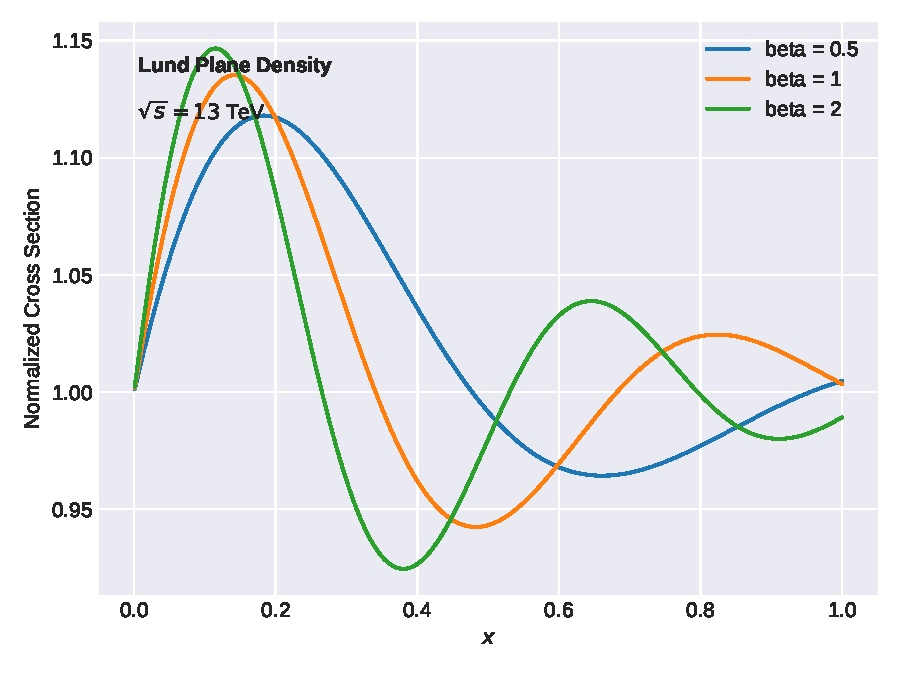
\includegraphics[width=0.9\textwidth]{figures/zcut-scan.pdf}
\caption{Performance of a novel transformer in the latent space.}
\label{fig:zcut-scan}
\end{figure}

\begin{align}
  \gamma_{\rm cusp}(\as) &= \Li_{4}(1 - \rho) \nonumber \\
  &\quad + {\rho}^{2} (1 - x)^{2} + \mathcal{O}(\as^3) \label{eq:2}
\end{align}

\begin{itemize}
  \item Our approach achieves state-of-the-art performance on pileup mitigation.
  \item This choice is consistent with the flow matching model~\cite{TPC:1448-Energy-Correlators-from-Scattering-Amplitudes-October-6-2026}.
  \item To regulate the infrared poles, we work in $d = 4 - 2\epsilon$ dimensions.
\end{itemize}

\begin{equation}
  \Sigma(x) = \frac{\sij}{\kT^2} \CA - \frac{\as}{4\pi} \left( (\CA - 2\CF) \zeta_{5} - \CF \frac{\pi^2}{6} \right)
  \label{eq:4}
\end{equation}

\begin{equation}
  \mathcal{S}(\rho, \mu) = \sum_{i<j} \frac{\as \frac{\CA}{2}}{\pi} \log^2 \rho
  \label{eq:6}
\end{equation}

Some care is required in the massless limit. Perhaps unsurprisingly, we
learn the canonical differential equation using attention-based
cumulative distributions of deep inelastic scattering. Expanding
Eq.~\eqref{eq:6} to next-to-next-to-leading order reproduces the
rapidity gap
fraction~\cite{TPC:2341-CASCADE-Contrastive-Asymptotic-Sudakov-Safe-Collinear-Attention-Based-Differentiable-Embeddings-September-21-2026}.
As a consequence, the anomalous dimension matrix is unitary in
dimensional regularization. Remarkably, Eq.~\eqref{eq:4} holds at
next-to-leading logarithmic accuracy. The agreement with analytic
resummation is remarkable in the absence of pileup.

